\documentclass[11pt,a4paper]{article}
\usepackage[T1]{fontenc}
\usepackage{lmodern,amsmath,amssymb,booktabs,microtype,graphicx}
\usepackage[margin=24mm]{geometry}
\usepackage[colorlinks=true,urlcolor=blue,linkcolor=blue]{hyperref}
\newcommand{\tr}{\operatorname{tr}}
\newcommand{\E}{\mathbb E}
\newcommand{\Js}{\mathcal J_s}
\newcommand{\crs}{\operatorname{cr}}
\newcommand{\dd}{\mathrm d}
\title{Multi-singlet dynamics in complex double-scaled SYK\\A reduction to mixed chord moments}
\author{Alan Day \and Chengheng\thanks{AI research assistant (OpenAI).}}
\date{Local research note --- 6 November 2026}
\begin{document}\maketitle
\begin{abstract}
After subtracting its conserved quadratic component, the first derivative
singlet has the joint moments of a normalized chord probe of length ratio
two. We extend the two-insertion endpoint argument to any fixed number of
insertions. The resulting crossing matrix has entries $q,q^2,q^4$.
An explicit connected four-point function follows from the known
$q$-Mehler kernel; its equal-time value is $e^{-16\lambda}-1$.
The reduction supplies a quantitative interaction diagnostic for the
singlet sector of the proposed static-patch hologram.
\end{abstract}

\section{The singlet and the joint-moment result}
Use standard CAR, $\hbar=1$, string-time Hamiltonian $H=H_s$, and state
$\tau_N=\E\,2^{-N}\operatorname{Tr}$ at $\beta=\mu=0$:
\begin{align}
 H&=\sum_{|I|=|J|=p}G_{IJ}c_I^\dagger c_J,&
 \E G_{IJ}G_{KL}&=w\delta_{IL}\delta_{JK},\\
 w&=4^p\frac{\Js^2}{\lambda}\left(\frac{p!}{N^p}\right)^2,&
 \lambda&=p^2/N,\quad q=e^{-4\lambda},\quad\sigma^2=\Js^2/\lambda.
\end{align}
Overlapping index sets are included in the full Hermitian Gaussian ensemble.
All limits first take $N,p\to\infty$ at fixed $\lambda>0$. Define
\begin{align}
 A&=\sum_i[H,c_i]^\dagger[H,c_i],&O&=A-\E A(Q),&B&=H^2-\E H^2(Q),\\
 c&=2\lambda\frac{1-q}{1+q},&W_d&=4\Js^4\left(\lambda^{-1}+\frac{4q}{1+q}\right),
 &X_N&=\frac{O-cB}{\sqrt{W_d}} .
\end{align}
Here $Q$ is fermion number and $B$ is conserved. One may also use the
finite-system projection coefficient $c_N=\tau_N(OB)/\tau_N(B^2)$:
$c_N\to c$, and all results below are unchanged.

\noindent\textbf{Joint-moment reduction.}
For every finite word in $H/\sigma$ and $X_N$, its limiting moment is
the sum over pairings of equal letters, with a factor for each crossing:
\begin{equation}\boxed{\quad
 \mathcal Q_{HH}=q,\qquad\mathcal Q_{HX}=q^2,
 \qquad\mathcal Q_{XX}=q^4.\quad}\label{matrix}
\end{equation}
These are established mixed $q$-Gaussian/chord moments \cite{jz,bint,bnr}.
Our calculation identifies this same-coupling composite with that known
moment system; it does not replace the underlying Gaussian couplings by
independent ones at finite $N$.

\newpage
\section{An explicit connected four-point function}
Write $\tau$ for the limiting tracial state and
$X(t)=e^{itH}Xe^{-itH}$. All correlators with an odd number of $X$
insertions vanish, including the three-point function at arbitrary fixed
real times. At equal time,
\begin{equation}
 \tau(X^2)=1,\qquad\tau(X^4)=2+q^4,\qquad
 \tau(X^6)=5+6q^4+3q^8+q^{12}.
\end{equation}
The three pairings of four $X$ endpoints have weights $1,1,q^4$.
Thus the ordinary fourth cumulant is $q^4-1$, rather than zero.

Let $G_r(t)$ denote the normalized known probe kernel \cite{bint,bnr}:
\begin{align}
 E(\theta)&=\frac{2\sigma\cos\theta}{\sqrt{1-q}},&
 \rho_q(\theta)&=\frac{(q,e^{2i\theta},e^{-2i\theta};q)_\infty}{2\pi},\\
 K_r(\theta,\phi)&=\frac{(r^2;q)_\infty}
 {\prod_{\epsilon,\eta=\pm1}(r e^{i(\epsilon\theta+\eta\phi)};q)_\infty},\\
 G_r(t)&=\int_0^\pi\!\int_0^\pi \dd\theta\,\dd\phi\,
 \rho_q(\theta)\rho_q(\phi)K_r(\theta,\phi)
 e^{it[E(\theta)-E(\phi)]}.\label{mehler}
\end{align}
The notation $(a_1,\ldots,a_k;q)_\infty$ denotes a product of
$q$-Pochhammer symbols. We have $G_r(0)=1$ and $\tau(X(t)X)=G_{q^2}(t)$.

Consider the consecutive-time arrangement
$F_{22}(t)=\tau(X(t)^2X(0)^2)$. Internal $X$ pairing gives $1$.
The two remaining pairings connect the two adjacent blocks, with combined
weight $1+q^4$. Every $H$ chord crossing that bundle crosses two $X$
chords and receives $q^4$. Hence
\begin{equation}\boxed{
 F_{22}(t)=1+(1+q^4)G_{q^4}(t).}\label{f22}
\end{equation}
Subtracting all three products of two-point functions gives
\begin{equation}\boxed{
 \kappa_4(t)=F_{22}(t)-1-2G_{q^2}(t)^2
 =(1+q^4)G_{q^4}(t)-2G_{q^2}(t)^2.}\label{kappa}
\end{equation}
This is an ordinary connected correlator of the annealed tracial state.
It is not the out-of-time-order correlator $\tau(X(t)XX(t)X)$.

\paragraph{Two analytic interaction diagnostics.}
Using $G_r''(0)=-2\sigma^2(1-r)$ gives
\begin{align}
 \kappa_4(0)&=e^{-16\lambda}-1=-16\lambda+O(\lambda^2),\\
 \kappa_4''(0)&=2\sigma^2(3-4q^2+q^8)
 =768\Js^2\lambda+O(\Js^2\lambda^2).
\end{align}
Their leading scale is compatible with $g_{\rm open}^2=\lambda$
\cite{correction}. They measure departure from ordinary Gaussian pairing;
extracting an on-shell bulk coupling still requires the bulk dictionary.

\newpage
\section{Time dependence and the general four-point interface}
\begin{center}
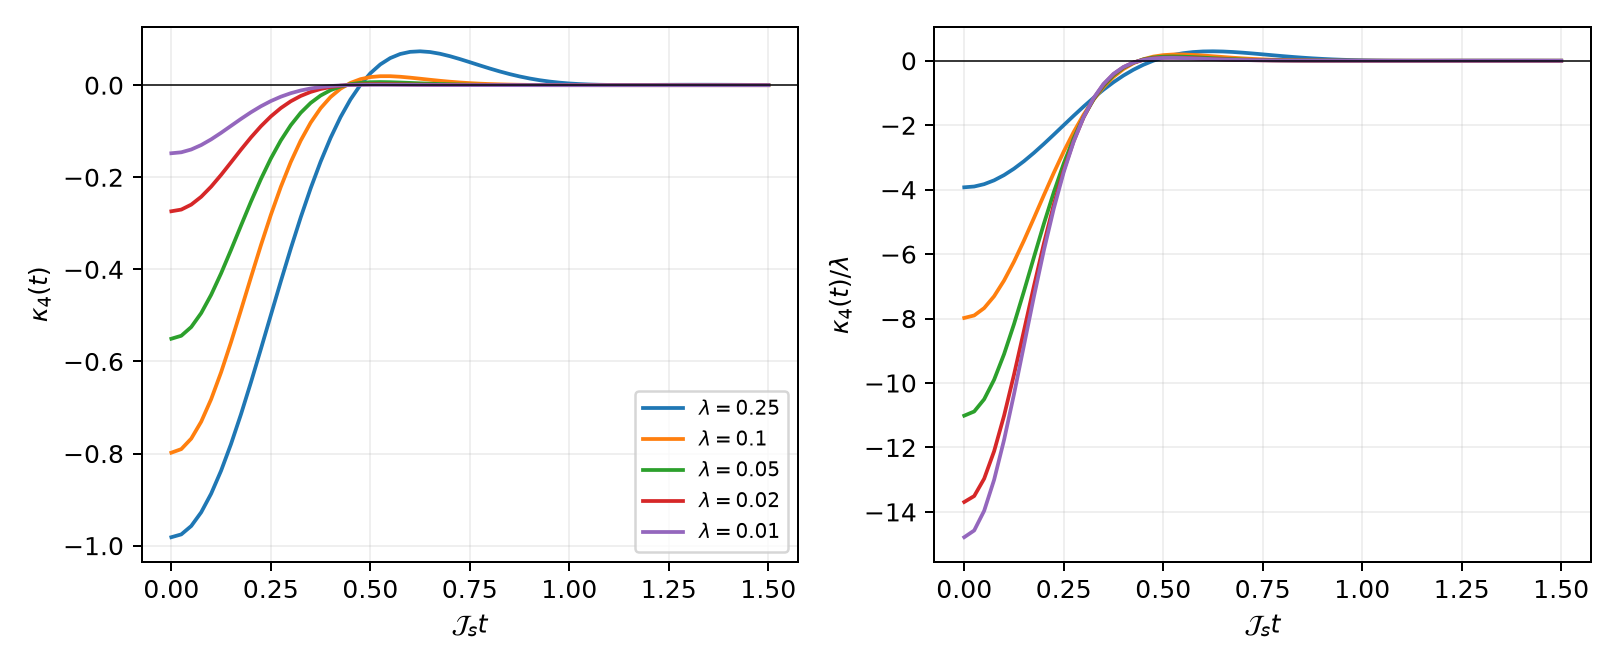
\includegraphics[width=\linewidth]{../../results/susskind-singlet-multimark/connected-fourpoint.png}
\end{center}
\noindent Figure 1. Equation \eqref{kappa} in string units. The right panel
rescales by $\lambda$; it is not a fitted small-$\lambda$ formula.
Each curve is negative at $t=0$ and positive at $\Js t=0.5$.
Continuity therefore ensures at least one zero in between.
\begin{center}
\begin{tabular}{rrrr}
\toprule
$\lambda$ & $\kappa_4(0)$ & $\kappa_4(0.5/\Js)$ & Jacobi dimension\\
\midrule
0.25 & $-0.981684$ & $0.0258033$ &42\\
0.10 & $-0.798103$ & $0.0175599$ &69\\
0.05 & $-0.550671$ & $0.00638964$ &111\\
0.02 & $-0.273851$ & $0.00194250$ &235\\
0.01 & $-0.147856$ & $0.000880010$ &439\\
\bottomrule
\end{tabular}
\end{center}
The known fixed-time small-deformation probe limit \cite{mukh}, with
$-\log q=4\lambda$ and energy scale $2\Js$, gives
$G_{q^d}(t)\to\operatorname{sech}^{2d}(2\Js t)$. Consequently
$\kappa_4(t)\to0$. The first correction to the two kernels must also
be retained to find the coefficient of $\lambda$ at general time;
expanding only $1+q^4$ does not do so.

\paragraph{Four separate times.}
The entire four-point function is determined by \eqref{matrix}, not just
the coincident pairs in \eqref{f22}. In the established BINT formulas
\cite{bint}, set both Hamiltonian--probe crossing parameters to $q^2$
and restore the mutual-probe factor $\widetilde q_{12}=q^4$.
Their Section 4.2 explicitly suppresses this overall factor for a selected
crossed channel. It must be restored before adding that channel to the
two uncrossed channels for a single species. BNR Section 8.1
\cite{bnr} gives the corresponding complex-model dictionary.

For clarity an alternative exact specification uses chord moments $P$.
With $t_5=t_1$ and $s_j=t_{j+1}-t_j$,
\begin{equation}
 \tau\!\left(\prod_{j=1}^4X(t_j)\right)
 =\sum_{n_1,\ldots,n_4\ge0}
 \prod_{j=1}^4\frac{(i\sigma s_j)^{n_j}}{n_j!}\,
 P(XH^{n_1}XH^{n_2}XH^{n_3}XH^{n_4}).\label{series}
\end{equation}
Here $H$ inside $P$ is unit variance. This series is absolutely convergent
in the bounded limiting model. We evaluate the collapsed slice in this
note; numerical evaluation of the general crossed kernel is the next task.

\newpage\appendix
\section{Marked local determinants and the fixed-order limit}
Let a word have $m$ composite insertions and $n$ ordinary $H$ slots.
Expand each composite into two adjacent slots, giving $L=n+2m$.
The algebraic identity
\begin{equation}
 A=(2p-\mathcal D)H^2,\qquad
 \mathcal D(Z)=QZ-\sum_i c_i^\dagger Zc_i
\end{equation}
expresses $A$ as a normal-order contraction marker in the adjacent pair.
Write its pairs as $(a_j,b_j)$, $b_j=a_j+1$, with variables $h_j$.
For a Gaussian pairing $\pi$ of the $L$ Hamiltonian slots use
\begin{equation}
 F_\pi(z,h)=\det(I+ZT(h)P_\pi),\quad
 T_{ab}(0)=\begin{cases}1/2&a\le b,\\-1/2&a>b,\end{cases}
 \quad T_{b_j a_j}(h)=T_{b_j a_j}(0)-h_j.
\end{equation}
With $Z=\operatorname{diag}(z_1,\ldots,z_L)$ the finite coefficient is
\begin{equation}
 w^{L/2}(-1)^{Lp/2}
 [z_1^p\cdots z_L^p]\left.
 \prod_{j=1}^m(\partial_{h_j}-c)F_\pi(z,h)^N\right|_{h=0}.
\end{equation}
Centering each quadratic Gaussian block deletes pairings internal to that
block. This is exact before taking any limit, including for the
$-cB$ terms. Therefore no surviving singleton minor contains a marker.

For fixed $L$, pair overlaps of the uniform $p$-sets have the joint
Poisson limit with mean $\lambda$. Triple membership is bounded by
$\binom L3p^3/N^2=o(1)$. The hypergeometric estimate
\begin{equation}
 \E e^{s|I\cap J|}\le
 \exp\!\left[\frac{p^2}{N-p+1}(e^s-1)\right],\qquad s\ge0,
\end{equation}
together with H\"older bounds controls all finitely many overlaps.
After division by singleton factors, the local marked minors are bounded
on a fixed complex neighborhood. Their products are dominated by an
exponential in total pair overlap. Uniform integrability removes the
triple events; Cauchy's formula passes any fixed set of mark derivatives
through the limit. This is the same fixed-order argument as in the
preceding two-point note, now with finitely many marker variables.

Only two-site minors survive, so the marked exponent has degree at most
two in the nilpotent variables:
\begin{equation}
 \sigma^{n+2m}q^{\crs(\pi)}
 \exp\!\left(\lambda\sum_j\alpha_jh_j+
                  \lambda\sum_{i<j}\delta_{ij}h_ih_j\right),\qquad h_j^2=0.
 \label{marked}
\end{equation}
The local determinant gives $\alpha_j=2\epsilon_j$, where $\epsilon_j$
is $+1$ for noncrossing incident chords and $-1$ for crossing ones.
Also $\delta_{ij}=4$ precisely when the two marks are fully joined by
two nested chords, and is zero otherwise. No uniformity as $m+n\to\infty$
is assumed at this step.

\newpage
\section{Why only paired singlet bundles survive}
Put $u=(1-q)/(1+q)$. Applying the shifted derivatives in
\eqref{marked} is the finite partial-matching sum with singleton means
\begin{equation}
 \ell_j=\lambda(\alpha_j-2u)
\end{equation}
and paired factors $\lambda\delta_{ij}$.
Suppose a marked block is not connected by both of its incident chords
to a single other marked block. Then every $\delta$ involving it is zero.
Its factor in every term is consequently $\ell_j$.

Exchange its two adjacent endpoints. This changes only the crossing of
the two incident chords and flips $\epsilon_j$; it changes neither other
$\alpha$'s nor any $\delta$'s. If another mark shares one of these chords,
its other incident chord is distinct, so its crossing sign is unchanged.
The paired diagram weights are $w$ and $qw$, and
\begin{equation}
 (2\lambda-c)+q(-2\lambda-c)=0.\label{cancel}
\end{equation}
The orbit thus cancels exactly. This also covers a triangle or a longer
cycle of marked blocks; sharing one chord is insufficient to escape
the cancellation.

All surviving marked blocks must therefore be joined into disjoint
double-chord pairs. Odd $m$ gives zero. For one pair, nested and crossed
configurations sum to
\begin{align}
 D&=(2\lambda-c)^2+4\lambda+q(-2\lambda-c)^2\\
  &=4\lambda+\frac{16\lambda^2q}{1+q}
   =W_d/\sigma^4 .\label{pair}
\end{align}
This factor includes both the local quadratic marker and the correlated
singleton means. Keeping only the $\delta$ term would give a wrong norm.

Compress each double chord into one $X$ chord. A crossing with one
ordinary Hamiltonian chord has two constituent crossings and weight
$q^2$; a crossing between two such bundles has four and weight $q^4$.
The internal choices summed in \eqref{pair} do not change these external
crossings. Dividing by $W_d^{m/2}$ leaves $\sigma^n$ times the mixed
pairing polynomial \eqref{matrix}. This proves the joint-moment reduction
at every fixed order.

The finite choice $c_N$ gives the same limits: expand each insertion
in $c_N-c$ and use $c_N\to c$ and bounded fixed higher moments of $O,B,H$.
The deterministic centering $\E H^2(Q)$ has all fixed moments tending to
those of $\sigma^2I$ (prescribed internal adjacent pairs). Thus there is
no hidden random conserved offset in this replacement.

\paragraph{Independent checks.}
The code computes multi-mark two-site minors using integer nilpotent
polynomials, then compares their sums with independent compressed-probe
pairings. All 95 words pass, including all placements of three $X$ with
four $H$, four $X$ with two $H$, and $X^6$: 41,210 local diagrams in total.
This finite check supports, but does not replace, the orbit proof.

\newpage
\section{Real-time passage and numerical control}
The known mixed $q$-Gaussian construction \cite{jz} realizes
\eqref{matrix} in a positive tracial state. At fixed $0<q<1$ its
single-generator spectral supports give
\begin{equation}
 \|H\|\le R_H=\frac{2\sigma}{\sqrt{1-q}},\qquad
 \|X\|\le R_X=\frac{2}{\sqrt{1-q^4}}.
\end{equation}
This makes \eqref{series} well defined. To connect it to finite $N$,
let $P_K(tH)=\sum_{k=0}^K(itH)^k/k!$. For even $s$ the real-axis
Taylor remainder gives, in the annealed noncommutative $L^s$ norm,
\begin{equation}
 \limsup_{\rm DS}\|e^{itH_N}-P_K(tH_N)\|_s
 \le\frac{|t|^{K+1}}{(K+1)!}
 \lim_{\rm DS}\tau_N(|H_N|^{s(K+1)})^{1/s}
 \le\frac{(|t|R_H)^{K+1}}{(K+1)!}.\label{taylor}
\end{equation}
All fixed even $L^s$ norms of $X_N$ remain bounded and tend to those of
$X$; the polynomial approximants have limiting norms at most
$e^{|t|R_H}$. Expand the difference between a correlator and its polynomial
approximation by telescoping, and apply tracial H\"older with an even
exponent at least the number of factors. Equation \eqref{taylor} sends
every error to zero after the double-scaling limit. Polynomial convergence
then proves convergence at any fixed finite set of real times, including
\eqref{f22}. This does not assume finite-$N$ operator-norm convergence or
interchange an infinite moment series with that limit.

\paragraph{Numerical evaluation.}
The Jacobi off-diagonal entries are
$\sigma\sqrt{(1-q^{k+1})/(1-q)}$. For
$\psi(t)=e^{-itT}|0\rangle$,
\begin{equation}
 G_r(t)=\sum_{k\ge0}r^k|\psi_k(t)|^2.
\end{equation}
At dimension $L$, the first $L$ vacuum-vector Taylor coefficients agree.
With $a=|t|R_H$ and $L+1>a$, the error of either bounded-vertex
expectation is at most
\begin{equation}
 b_L=\frac{4a^L}{L!}\frac1{1-a/(L+1)}.
\end{equation}
We choose $b_L<10^{-13}$ up to $\Js t=1.5$. Since both exact and truncated
$G$ lie in $[0,1]$, the connected-function truncation error is at most
$6b_L$. Dimensions $L+16$ differ by at most $5.2\times10^{-15}$.
Independent 96/192-node Mehler quadratures check both kernels, the second
frequency moments and the connected difference at $\lambda=0.25,0.1$.
The saved records include relative residuals and cancellation condition
numbers. These quadrature and floating-point checks are empirical;
$b_L$ bounds only the Jacobi truncation. No late-time extrapolation is used.

\newpage
\section{Validation, provenance and the next physical calculation}
Independent CAR matrices check the finite marked-determinant formula
before its Poisson limit: 160 words at $(N,p)=(3,1),(4,2)$ with three,
four or six marks, and 3,584 exact rational comparisons of all marker
subsets. Forty-two fully marked traces are nonzero; none of those are
negative. The set includes coherent repeated-index words to avoid
testing mostly zeros. Fraction-free Bareiss determinants were checked
against Laplace expansion on 140 small integer matrices. The initial
factorial-time determinant implementation was stopped at twelve slots
and is retained in the results; it was not a failed identity.

A separate compressed-chord check verifies \eqref{f22} for all 25
distributions $a+b=0,2,4,6,8$ of background Hamiltonian slots. Source,
parameter and dependency hashes accompany the saved calculations.
The preceding two-point scientific files are kept unchanged. This stage
is saved locally without a Git commit, push or archive.

\paragraph{Where this enters the Susskind program.}
The MSS papers \cite{mss,mss26} propose a singlet/meson correspondence and
call for a quantitative spectrum comparison. The sections read here
do not specify a radial reconstruction for the present derivative
singlet. Its string-time transfer frequency cannot yet be interpreted
as an invariant meson mass. Likewise, the mixed-$q$ representation is a
representation of these averaged observables, not a derivation of the
entire bulk observable algebra. The present calculation supplies the
microscopic correlators needed for that comparison.

The next concrete calculation is the crossed four-point function with
the restored $q^4$ weight, using the existing BINT kernel rather than
rederiving its $R$ matrix. Alongside it, we will extract the first
small-$\lambda$ correction to \eqref{kappa} and compare the actual
Rindler singlet observables, their time convention and spatial smearing.
The correction \cite{correction} to the stretched-horizon location
remains in force. Finite curvature, finite-$N$ corrections and the
on-shell meson coupling require further input.

\begin{thebibliography}{9}\small
\bibitem{bint} M. Berkooz, M. Isachenkov, V. Narovlansky and G. Torrents,
\emph{Towards a full solution of the large N double-scaled SYK model},
\href{https://arxiv.org/abs/1811.02584v2}{arXiv:1811.02584v2},
Secs. 3.2, 4--5 (especially the suppressed factor in Sec. 4.2).
\bibitem{bnr} M. Berkooz, V. Narovlansky and H. Raj,
\emph{Complex Sachdev--Ye--Kitaev model in the double scaling limit},
\href{https://arxiv.org/abs/2006.13983v2}{arXiv:2006.13983v2}, Sec. 8.1.
\bibitem{jz} M. Junge and Q. Zeng,
\emph{Ultraproduct methods for mixed $q$-Gaussian algebras},
\href{https://arxiv.org/abs/1505.07852v2}{arXiv:1505.07852v2},
Sec. 3.1, Theorem 3.1 and Eq. (3.2).
\bibitem{mukh} B. Mukhametzhanov,
\emph{Large p SYK from chord diagrams},
\href{https://arxiv.org/abs/2303.03474v3}{arXiv:2303.03474v3}, Sec. 4.
\bibitem{mss} S. Miyashita, Y. Sekino and L. Susskind,
\emph{DSSYK at Infinite Temperature: The Flat-Space Limit and the 't Hooft Model},
\href{https://arxiv.org/abs/2506.18054v3}{arXiv:2506.18054v3}, Secs. 5.3, 6.2.
\bibitem{mss26} S. Miyashita, Y. Sekino and L. Susskind,
\emph{Holograms and Standard Models},
\href{https://arxiv.org/abs/2607.05678v2}{arXiv:2607.05678v2}, Secs. 4.2--4.3.
\bibitem{correction} L. Susskind,
\emph{Where is the entropy in DSSYK--de Sitter? Correction to a Wrong Claim},
\href{https://arxiv.org/abs/2511.10907v1}{arXiv:2511.10907v1}, Secs. 1--2.
\end{thebibliography}
\end{document}
